
\begin{equation}
\begin{aligned}
    \omega = u_r - u_l = K_\psi (\theta^R-\theta)& , \quad v = \frac{u_r + u_l}{2}= 0 \\
    u_r = \frac{K\psi(\theta^R - \theta)}{2}&, \quad u_l = - u_r
\end{aligned}
\end{equation}

Simulation results using $K_\psi=5$.

\begin{figure}[H]
    \centering
    \begin{subfigure}[b]{7cm}
        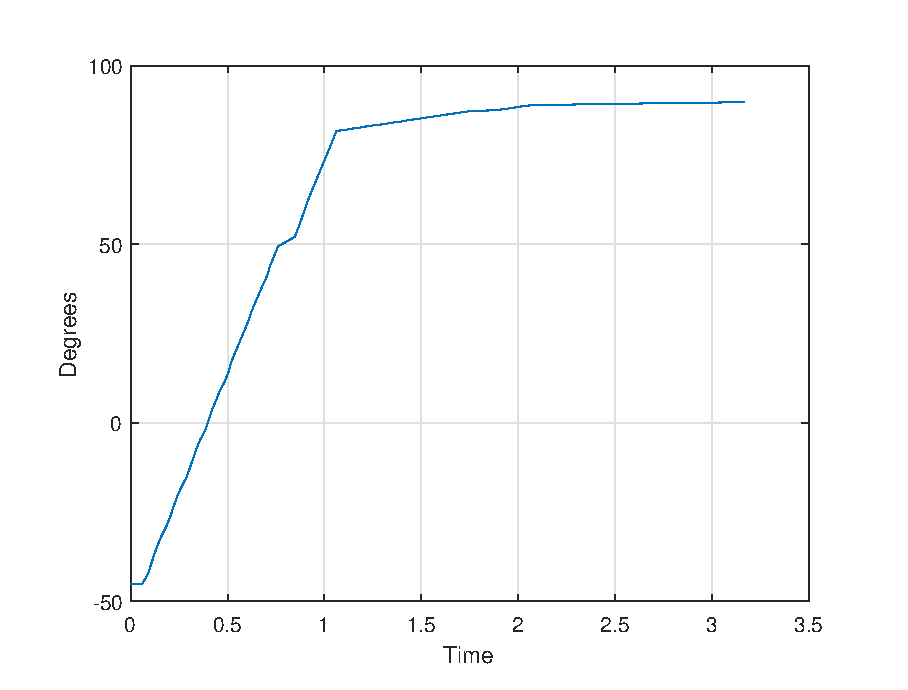
\includegraphics[width=\textwidth]{rotation_m45.eps}
        \caption{Initial angle: -45 degrees}
        \label{fig:m45deg}
    \end{subfigure}
    \begin{subfigure}[b]{7cm}
        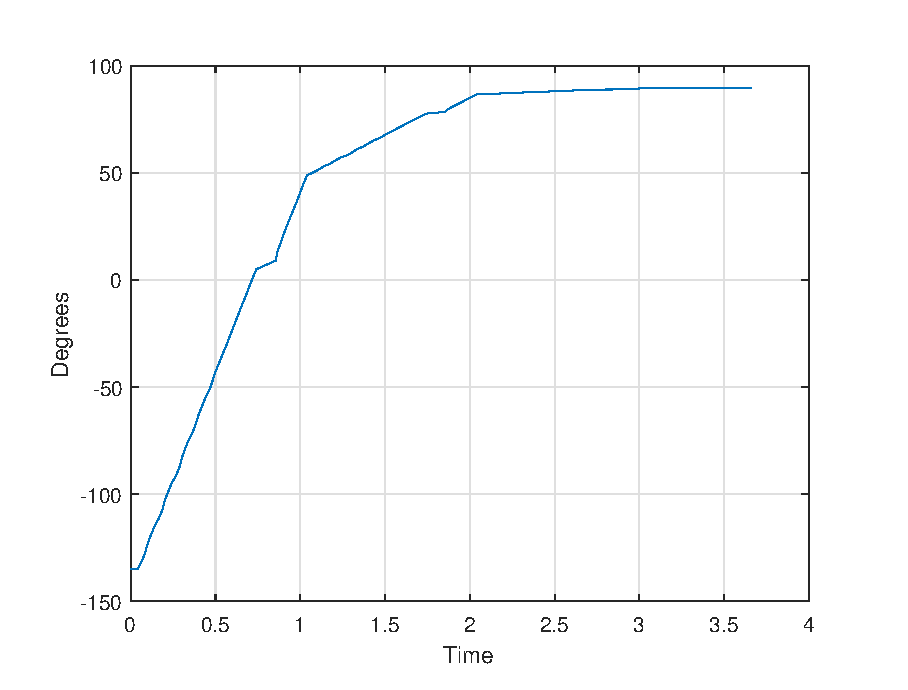
\includegraphics[width=\textwidth]{rotation_m135.eps}
        \caption{Initial angle: -135 degrees}
        \label{fig:m135deg}
    \end{subfigure}
   
   
    \begin{subfigure}[b]{7cm}
        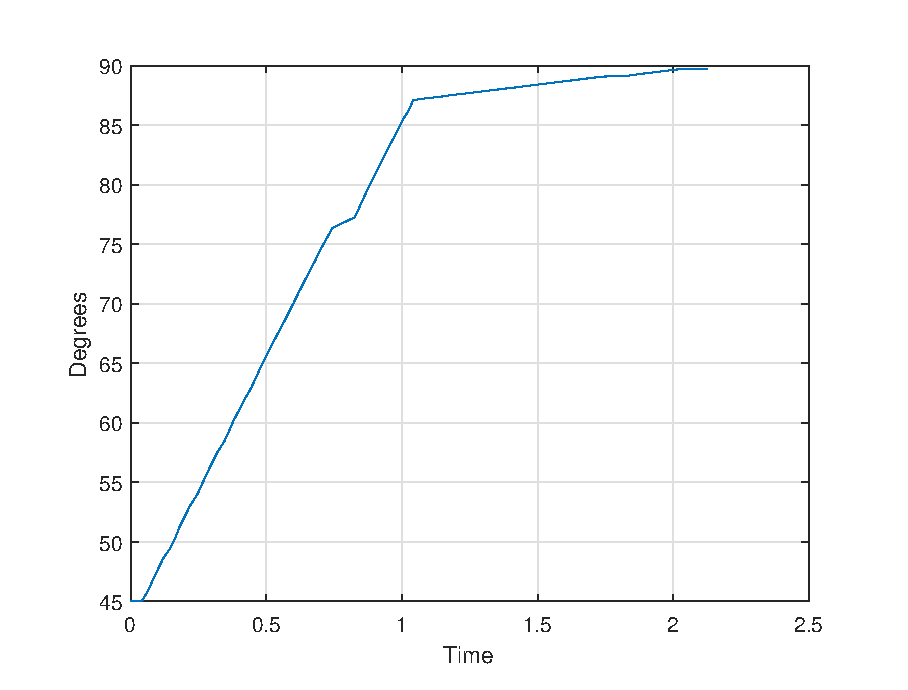
\includegraphics[width=\textwidth]{rotation_p45.eps}
        \caption{Initial angle: 45 degrees}
        \label{fig:45deg}
    \end{subfigure}
     \begin{subfigure}[b]{7cm}
        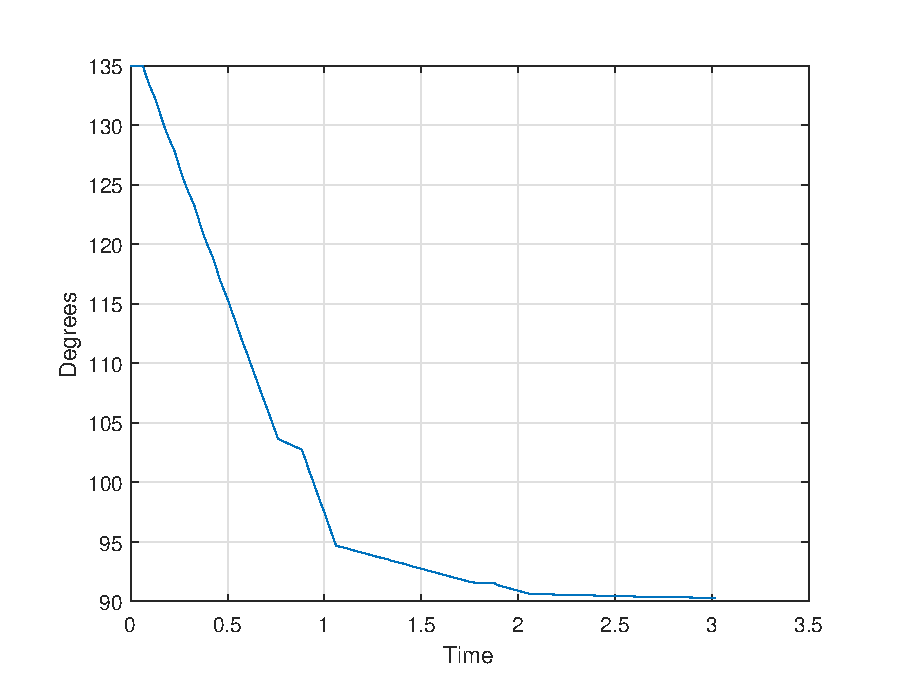
\includegraphics[width=\textwidth]{rotation_p135.eps}
        \caption{Initial angle: 135 degrees}
        \label{fig:135deg}
    \end{subfigure}
    \caption{Rotation, $K_\psi=5$, $\theta^R=90$ degrees}\label{fig:animals}
    \label{fig:dir-ctrl}
\end{figure}

As shown in task 5 it should be possible to maintain $\theta[k]$ at $\theta^R.$ However this does not account for the quantization error, which exists in both the measurements and the output, which might introduce a small offset. Task 5 does not account for any constant disturbances either, which would require an I controller to fix. It also assumes that the output will be constant during the time between samples. In all the plots in Fig \ref{fig:dir-ctrl} a small decrease in angular velocity can be seen at around $0.75$ seconds after each sample. This will slow down the controller and might make $\theta[k]$ go towards $\theta^R$ asymptotically, but not reaching it in finite time. 
%\begin{equation}
%\begin{aligned}
%    \omega = \dot{\theta} = K_\psi(\theta^R-\theta)  \Rightarrow \\
%    \dot{\theta} + K_\psi \theta - K_\psi \theta_\psi = 0 \Rightarrow \\
%    \theta = \theta^R + C e^{-K_\psi t}  \Rightarrow \\
%    \theta \rightarrow \theta^R \textrm{ as } t \rightarrow \infty
%\end{aligned}
%\end{equation}
%So it is possible to maintain $\theta=\theta^R$. 